\documentclass[12pt]{article}
\usepackage{geometry}
\geometry{a4paper}
\usepackage[round, sort]{natbib}
\usepackage{graphicx}
\usepackage[T1]{fontenc}
\usepackage[utf8]{inputenc}
\usepackage{textcomp}
\usepackage{gensymb}
\usepackage{amsmath}
\usepackage{amssymb}
\usepackage{authblk}
\usepackage[running]{lineno}
\usepackage{setspace}
\usepackage{longtable}
\usepackage{hyperref}
\usepackage{times}


\topmargin 0.0cm
\oddsidemargin 0.2cm
\textwidth 16cm
\textheight 21cm
\footskip 1.0cm

\doublespacing

\renewcommand\Authfont{\fontsize{12}{14.4}\selectfont}
\renewcommand\Affilfont{\fontsize{10}{10.8}\itshape}




\title{\normalsize CentralRange }

\author[a,*]{Grant Foster}

\author[a,*]{Tad A Dallas}


\affil[a]{Department of Biological Sciences, University of South Carolina, Columbia, SC, 29208 }



\renewcommand\Authands{ and }
\date{ \small *Corresponding author: AUTHOREMAIL@mailbox.sc.edu or gmail.com}



%% Potential reviewers
% Names and email addresses of potential reviewers
%
%
%
%
%
%






\begin{document}


\maketitle

\setstretch{1}
\vspace{-1cm}
\noindent \textbf{Running title}:\\


\noindent \textbf{Author contributions}: All authors contributed to manuscript writing. \\


\noindent \textbf{Acknowledgements}: This work has been supported by ... .  \\


\noindent \textbf{Data accessibility}: $R$ code is available on figshare at \\ \texttt{https://doi.org/ }. \\


\noindent \textbf{Keywords}:  \\

\noindent \textbf{Conflict of interest}: The authors have no conflicts of interest to declare.\\




\clearpage

\linenumbers


\noindent {\large TITLE}

\setstretch{1.3}


\subsection*{Abstract}




















\clearpage

\setstretch{1.3}
\subsection*{Introduction}

\paragraph*{}



\paragraph*{}






\paragraph*{}




% thesis
\paragraph*{}













%----------
\subsection*{Methods}

\paragraph*{Data}




\paragraph*{Species Ranges}
  We constructucted a global pollinator metaweb was created by querying Mangel for plant-pollinator networks. This resulted in a total of 65 globally distributed networks, and a total of 1018 individual species. For each species, we queried global occurance records from GBIF using the \texttt{rgbif} packages. Occurance points were first processed using \texttt{coordinateCleaner}; points were removed if they were present outside of the fossil record, occured within 2km of country centroids, were located on ocean, or were marked as an "introduced" individual.
\paragraph{}To avoid overestimating species range through including spurrious or transient records in GBIF, we used a quantile approach to filter out rare occurances.We projected the remaining occurance points onto a raster of terrestrial climate at a resolution 10 minutes, where each cell was assigned a value equal to the number of occurances in that cell. We then filtered occurance cells to only include occruance cells in the top 0.9 quantile of of number of records, and used only these top 10\% of occurance localities to estimate species range.
\paragraph{} Species ranges were calculated through both minimum convex polygon and alpha hull approaches ($\alpha = 20$). Each species range was calculated seperately for each continent according to a 7 continent model (Asia, Europe, Africa, Oceania, North America, Antartica, and South America); total species range was calculated as the total terrestrial area occupied across all continents.

\begin{figure}[h!]
  \begin{center}
    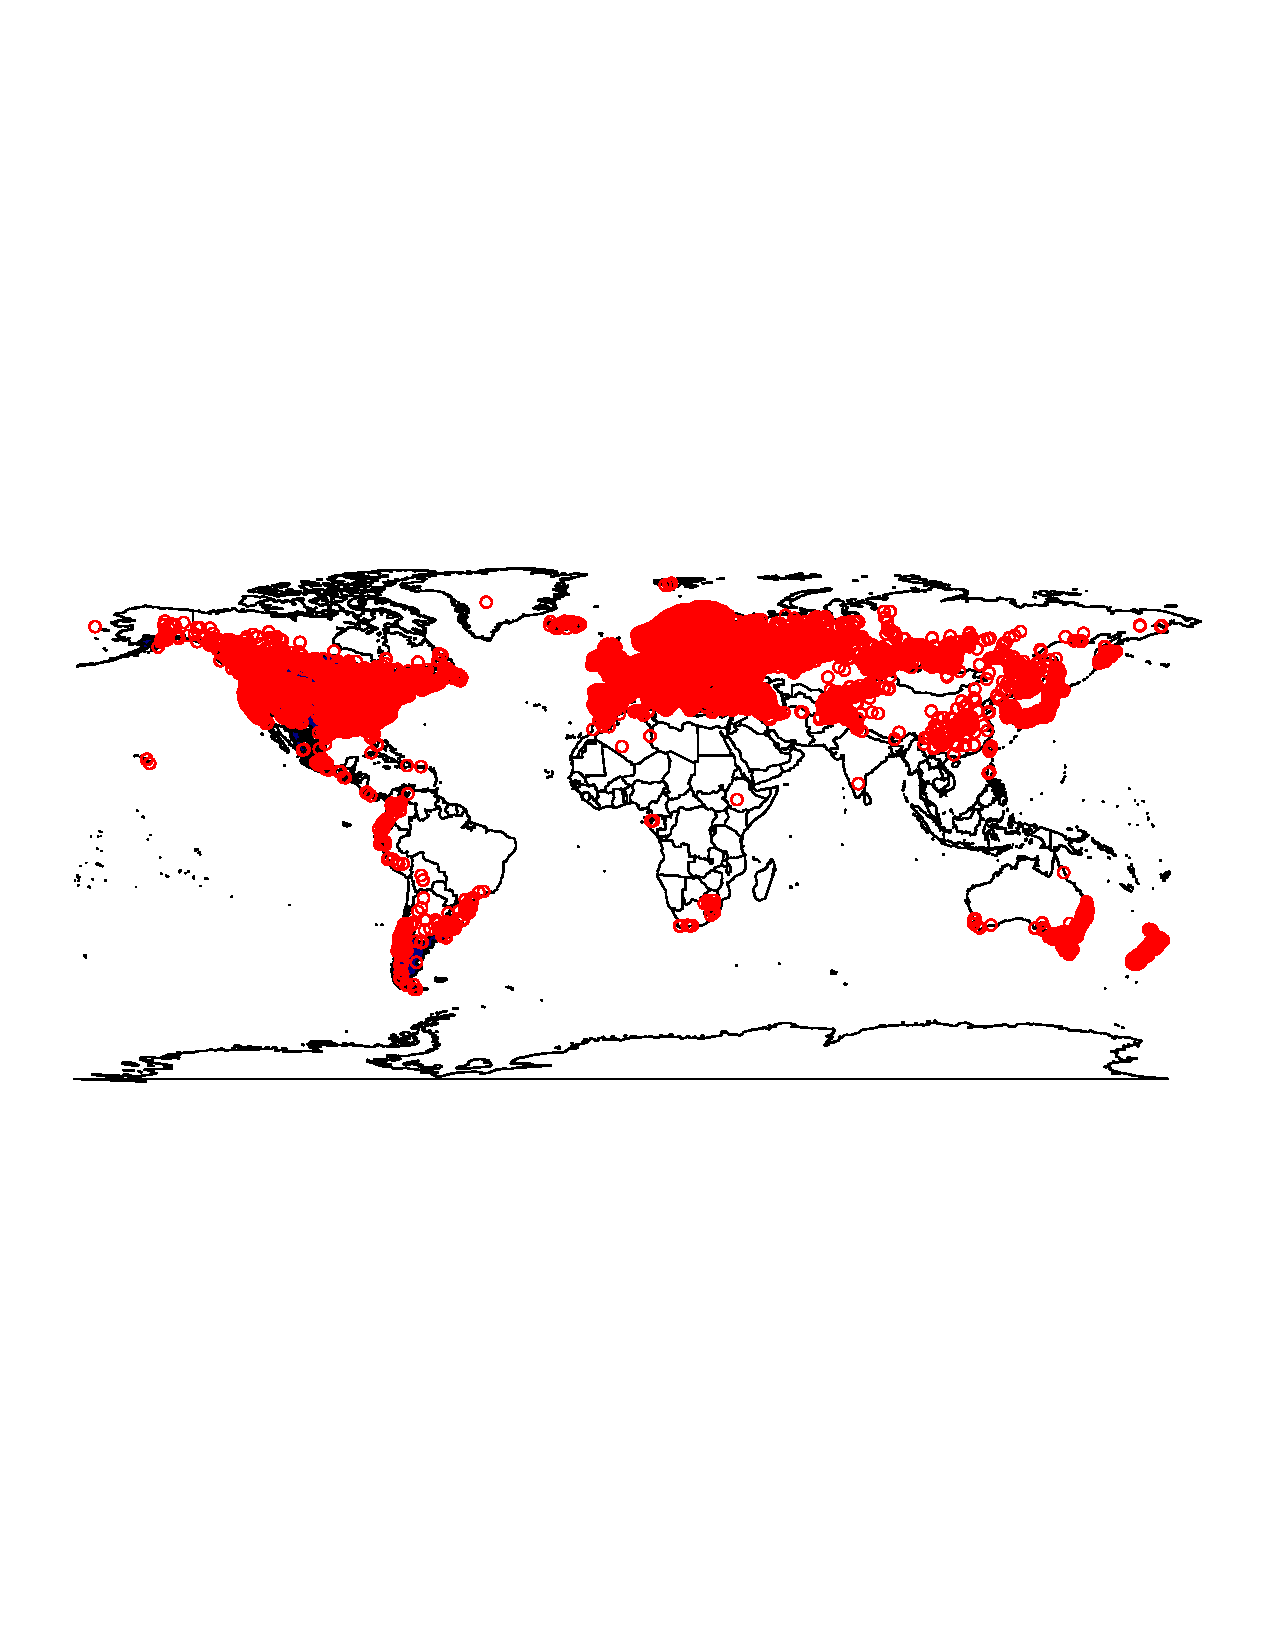
\includegraphics[width=\textwidth]{../analysis/figs/mapping/rawClover.pdf}
    \caption{Raw GBIF occurance points for red clover}
    \label{fig:fig1}
  \end{center}
\end{figure}


\begin{figure}[h!]
  \begin{center}
    %\includegraphics[width=\textwidth]{Figures/concept.pdf}
    \caption{A figure with caption. }
    \label{fig:fig2}
  \end{center}
\end{figure}


\begin{figure}[h!]
  \begin{center}
    %\includegraphics[width=\textwidth]{Figures/concept.pdf}
    \caption{A figure with caption. }
    \label{fig:fig3}
  \end{center}
\end{figure}






\paragraph*{Reproducibility}
$R$ code and data to reproduce the analyses is provided at \\
\texttt{https://doi.org/}























% -------------------
\subsection*{Results}


\paragraph*{}



\paragraph*{}



\paragraph*{}























% -------------------
\subsection*{Discussion}

\paragraph*{}



\paragraph*{}



\paragraph*{}



\paragraph*{}



\paragraph*{}








\paragraph*{}




















\clearpage

\bibliography{var}
\bibliographystyle{jae}







\clearpage
\subsection*{Tables}


\begin{table}[ht]
\centering
\caption{A table with caption. }
\label{tab:moran}
\begin{tabular}{lllllll}
  \hline
  covariate & t-SNE axis & obs & exp & sd & $p$-value & $z$-score \\
  \hline
  geography       & 1 & 0.02963 & -0.00032 & 0.00014 & \textbf{$<$ 0.0001} & 216.3 \\
                  & 2 & 0.01930 & -0.00032 & 0.00014 & \textbf{$<$ 0.0001} & 141.7 \\
  age structure   & 1 & 0.00043 & -0.00032 & 0.00001 & \textbf{$<$ 0.0001} & 60.5  \\
                  & 2 & 0.00017 & -0.00032 & 0.00001 & \textbf{$<$ 0.0001} & 39.4  \\
  population size & 1 & 0.00002 & -0.00032 & 0.00003 & \textbf{$<$ 0.0001} & 11.7  \\
                  & 2 & 0.00004 & -0.00032 & 0.00003 & \textbf{$<$ 0.0001} & 12.3  \\
  $R_0$           & 1 & 0.00339 & -0.00032 & 0.00003 & \textbf{$<$ 0.0001} & 110.7 \\
                  & 2 & 0.00135 & -0.00032 & 0.00003 & \textbf{$<$ 0.0001} & 49.8  \\

 \hline
\end{tabular}
\end{table}







\clearpage
\subsection*{Figures}

\begin{figure}[h!]
  \begin{center}
    %\includegraphics[width=\textwidth]{Figures/concept.pdf}
    \caption{A figure with caption. }
    \label{fig:concept}
  \end{center}
\end{figure}


























\clearpage

\newcommand{\beginsupplement}{%
        \setcounter{page}{1}
        \setcounter{table}{0}
        \renewcommand{\thetable}{S\arabic{table}}%
        \setcounter{figure}{0}
        \renewcommand{\thefigure}{S\arabic{figure}}%
        }

\section*{Supplementary materials}

\begin{center}
\textbf{Title}:       \\
\textbf{Authors}:     \\
\end{center}

\beginsupplement


\subsubsection*{}


\begin{figure}[h!]
  \begin{center}
    %\includegraphics[width=0.75\textwidth]{Figures/.pdf}
    \caption{Caption }
    \label{fig:label}
  \end{center}
\end{figure}










\end{document}
